\section{Observation and Calculations}

The resistance values are measured to be 9.81k$\Omega$, 9.94k$\Omega$, 0.999 k$\Omega$ and 0.999 k$\Omega$. Hence the average value of $R_1 = 9.875$ k$\Omega$ and $R_2 = 0.999$ k$\Omega$.

The capacitances used are 10.87nF and 10.91nF. The power supplied to the IC 741 opamp are roughly $\pm$15 V.
The amplitude of the AC wave is 1.000V (pp) and the frequency is 5.000 kHz. Dielectric Constant of the solar cell $\epsilon_s$ is 11.7. The area of the solar cell was measured to be $5.2 \times 3.6$ cm$^2$.

\subsection{Dark Environment}
The observed values of $V_{DC}$,$V_{DUT}$ and $V_{OUT}$ are shown in Table I.
Using the parameters above and Eq. 5, $C_{DUT}$ was calculated and was plotted as shown.

\begin{table}[H]
    \centering
    \begin{tabular}{|c|c|}
    \hline
    $V_{PMT}$ (mV) & $I_{PMT}$ (A) \\ \hline
    0.5 & 0.0 \\
    0.6 & 0.2 \\
    0.7 & 0.8 \\
    0.8 & 1.4 \\
    0.9 & 6.2 \\
    1.0 & 14.1 \\ \hline
\end{tabular}
\caption{Dark current vs supply voltage in PMT}
\end{table}

\begin{figure}
    \centering
    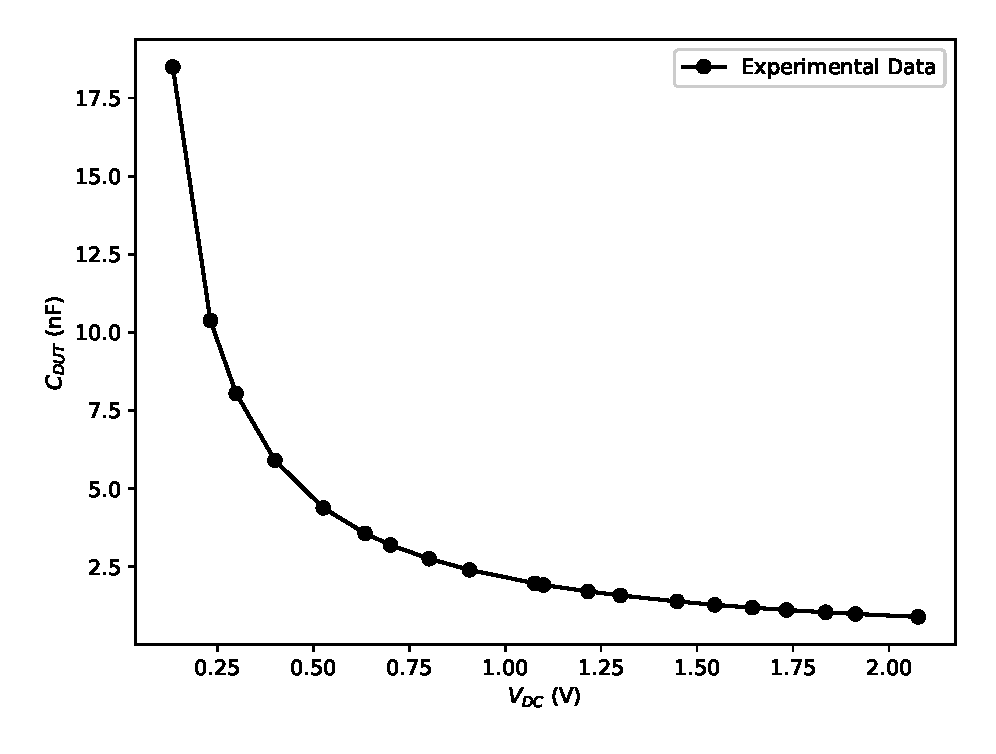
\includegraphics[width=1\columnwidth]{images/dark0.eps}
    \caption{Plot of $C_{DUT}$ vs $V_{DC}$ for dark condition}
\end{figure}

The curve in the above figure is clearly non linear The region of interest is the region in which
the $1/C^2_{DUT}$ vs $V_{DC}$ behaves almost linearly.

Now, consider Eq. 3, which can be rewritten as,

\begin{align}
    \frac{1}{C^2} &= \left(\frac{2}{q\epsilon_0\epsilon_sA^2}\right)\frac{V_{DC}}{N_d} + \left(\frac{2}{q\epsilon_0\epsilon_sA^2}\right)\frac{V_{bi}}{N_d} \nonumber\\
    \frac{1}{C^2} &= \alpha\frac{V_{DC}}{N_d} + \alpha\frac{V_{bi}}{N_d}
\end{align}

Here, $\alpha = \frac{2}{q\epsilon_0\epsilon_sA^2}$ is constant for all values of $C_{DUT}$ and $V_{DC}$. The above equation is of the form of a straight line. Hence plotting $1/C^2_{DUT}$ vs $V_{DC}$ and using linear regression to fit a straight line through the linerar region, we can calculate $N_d$ and $V_{bi}$. 

\begin{figure}
    \centering
    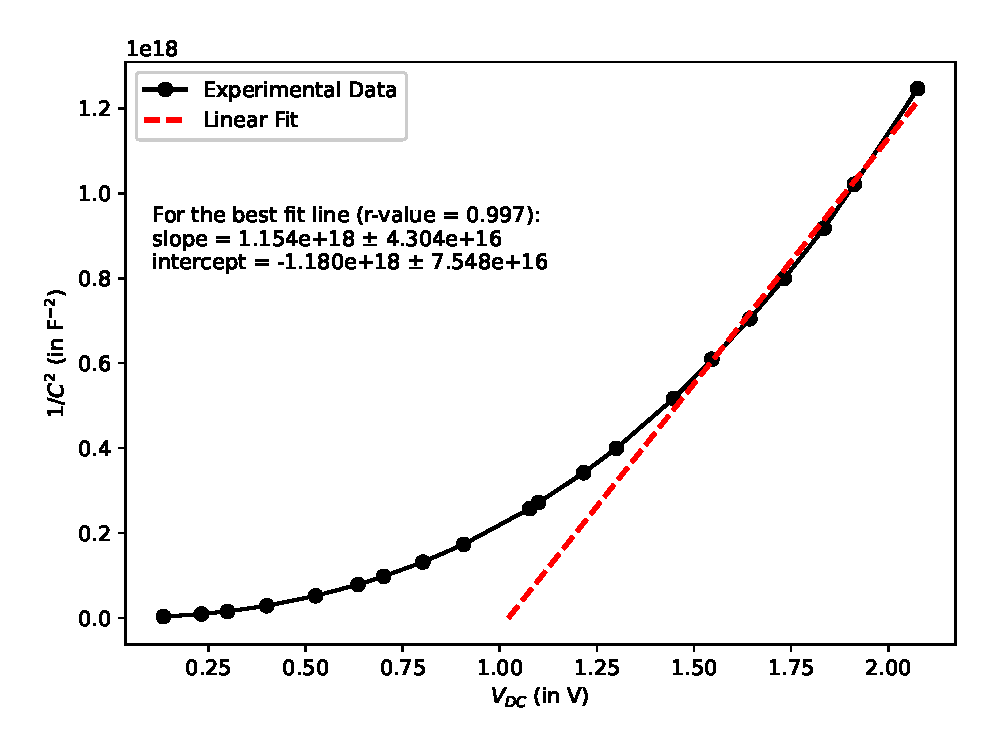
\includegraphics[width=1\columnwidth]{images/dark.eps}
    \caption{Plot of $1/C_{DUT}^2$ vs $V_{DC}$ for dark condition}
\end{figure}

Plugging in the values,
\begin{align*}
    \text{slope} &= \left(\frac{2}{q\epsilon_0\epsilon_sA^2}\right)\frac{1}{N_d}\\
    \implies N_d &= 2.984 \times 10^{16} \text{ m}^{-3}
\end{align*}

And, from the y-intercept (ignoring the negative sign),
\begin{align*}
    \text{intercept} &= \left(\frac{2}{q\epsilon_0\epsilon_sA^2}\right)\frac{V_{bi}}{N_d}\\
    \implies V_{bi} &= 1.022 \text{ V}
\end{align*}

Note that $V_{bi}$ is also the value of the x-intercept of the above plot.

\subsection{In Ambient Light}
The observed values of $V_{DC}$,$V_{DUT}$ and $V_{OUT}$ are shown in Table II.
Using the parameters above and Eq. 5, $C_{DUT}$ was calculated and was plotted as shown.

\begin{table}[]
    \centering
    \begin{tabular}{|c|c|c|c|}
    \hline
    $V_{DC}$ & $V_{DUT}$ & $V_{OUT}$ & $C_{DUT}$ \\ 
    (V) & (V) & (V) & (nF) \\  \hline
    0.117 & 0.117 & 0.248 & 23.698 \\ \hline
    0.26 & 0.259 & 0.242 & 10.446 \\ \hline
    0.419 & 0.416 & 0.238 & 6.396 \\ \hline
    0.511 & 0.51 & 0.234 & 5.130 \\ \hline
    0.625 & 0.624 & 0.231 & 4.139 \\ \hline
    0.751 & 0.749 & 0.227 & 3.388 \\ \hline
    0.878 & 0.873 & 0.224 & 2.869 \\ \hline
    1.053 & 1.052 & 0.219 & 2.327 \\ \hline
    1.139 & 1.137 & 0.217 & 2.134 \\ \hline
    1.205 & 1.203 & 0.215 & 1.998 \\ \hline
    1.32 & 1.318 & 0.214 & 1.815 \\ \hline
    1.407 & 1.406 & 0.212 & 1.686 \\ \hline
    1.571 & 1.569 & 0.208 & 1.482 \\ \hline
    1.669 & 1.667 & 0.207 & 1.388 \\ \hline
    1.735 & 1.732 & 0.206 & 1.330 \\ \hline
    1.829 & 1.825 & 0.204 & 1.250 \\ \hline
    1.91 & 1.908 & 0.203 & 1.190 \\ \hline
    2.048 & 2.045 & 0.200 & 1.093 \\ \hline
    \end{tabular}
    \caption{Data for study of CV characteristics of solar
    cell in ambient light conditions}
    \label{tab:2}
\end{table}

\begin{figure}
    \centering
    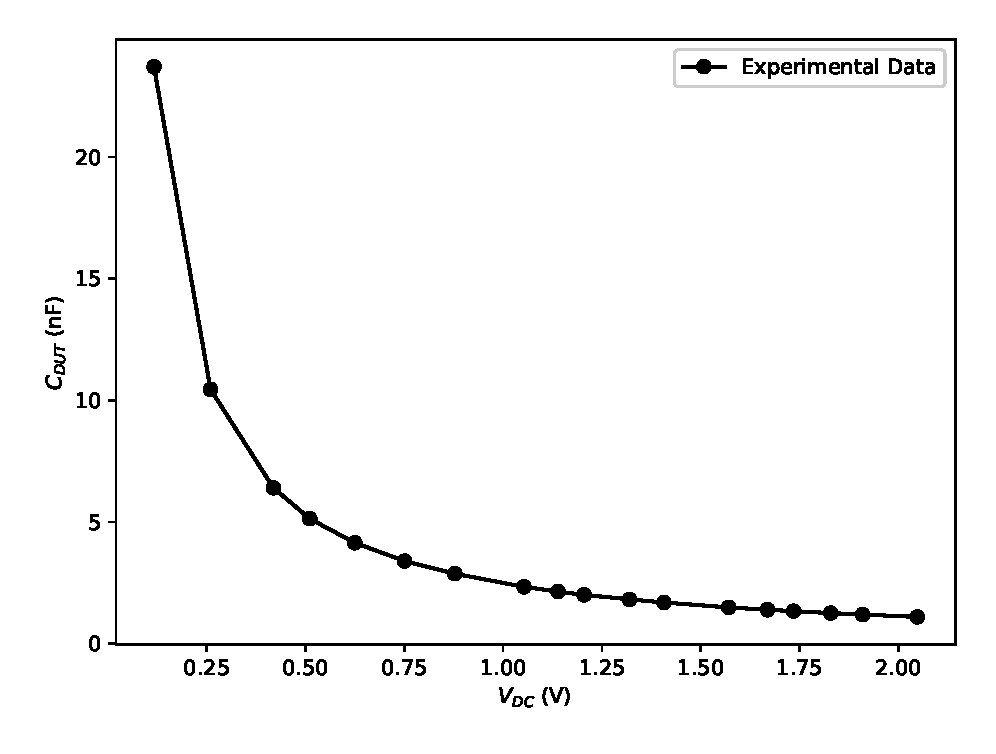
\includegraphics[width=1\columnwidth]{images/light0.eps}
    \caption{Plot of $C_{DUT}$ vs $V_{DC}$ for light condition}
\end{figure}

Similarly to the dark condition, a linear fit was performed on the linear region of the $1/C_{DUT}^2$ vs $V_{DC}$ plot.

Plugging in the values,
\begin{align*}
    \text{slope} &= \left(\frac{2}{q\epsilon_0\epsilon_sA^2}\right)\frac{1}{N_d}\\
    \implies N_d &= 4.588 \times 10^{16} \text{ m}^{-3}
\end{align*}

And, from the y-intercept,
\begin{align*}
    \text{intercept} &= \left(\frac{2}{q\epsilon_0\epsilon_sA^2}\right)\frac{V_{bi}}{N_d}\\
    \implies V_{bi} &= 0.963 \text{ V}
\end{align*}

\begin{figure}
    \centering
    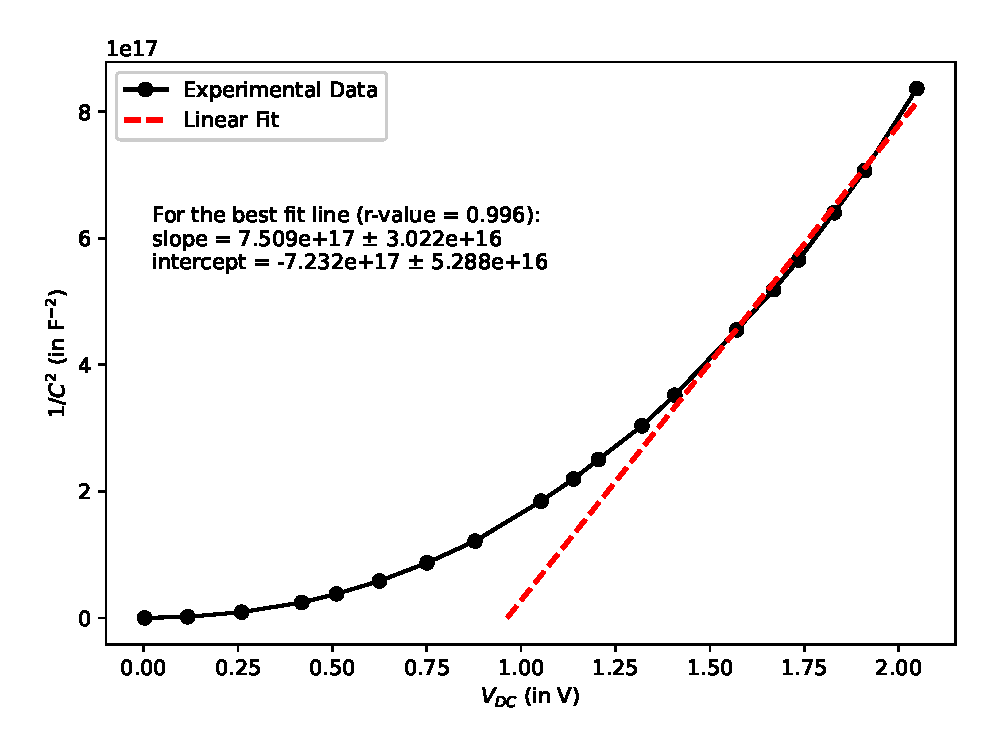
\includegraphics[width=1\columnwidth]{images/light.eps}
    \caption{Plot of $1/C_{DUT}^2$ vs $V_{DC}$ for light condition}
\end{figure}

\section{Error Analysis}

From Eq. 6, the error in $\alpha$ can be calculated Using

\begin{align}
    \Delta \alpha = \alpha \left(\frac{2 \Delta A}{A}\right)
\end{align}

since $A$ is the only measured parameter. Using $\Delta A = 0.01$ cm$^2$ and $\alpha = 3.445 \times 10^{34}$ C$^{-1}$ F$^{-1}$ m$^{-3}$, we get $\Delta \alpha = 3.680 \times 10^{31}$ C$^{-1}$ F$^{-1}$ m$^{-3}$.

The error in $N_d$ and $V_{bi}$ can be calculated using,

\begin{align}
    \Delta N_d &= N_d \sqrt{\left(\frac{\Delta \text{slope}}{\text{slope}}\right)^2 + \left(\frac{\Delta \alpha}{\alpha}\right)^2}\\
    \Delta V_{bi} &= V_{bi} \sqrt{\left(\frac{\Delta \text{intercept}}{\text{intercept}}\right)^2 + \left(\frac{\Delta \alpha}{\alpha}\right)^2 + \left(\frac{\Delta N_d}{N_d}\right)^2}
\end{align}

These come out to be,

\begin{itemize}
    \item Dark conditions,
    \begin{align*}
        \Delta N_d &= 0.111 \times 10^{16} \text{ m}^{-3}\\
        \Delta V_{bi} &= 0.076 \text{ V}
    \end{align*}
    \item Ambient conditions,
    \begin{align*}
        \Delta N_d &= 0.185 \times 10^{16} \text{ m}^{-3}\\
        \Delta V_{bi} &= 0.080 \text{ V}
    \end{align*}
\end{itemize}

